\chapter{Resultados}

	El presente capítulo expone los resultados obtenidos tras el desarrollo del sistema de desalinización propuesto. Los resultados se organizan para proporcionar una visión integral del diseño y funcionamiento del sistema. Para lograr este cometido, se presenta de manera coherente de acuerdo al proceso seguido para obtener estos resultados.
	
	En primer lugar, se muestra la vista general del funcionamiento del sistema para comprender la interacción entre los componentes del desalinizador. A continuación, se entra en detalle con el diseño propuesto y se validan los componentes a través de simulaciones de transferencia de calor que sustentarán al modelo de control difuso que regula la alimentación del sistema.

	
	\section{Comportamiento e interacciones del desalinizador propuesto}
	
		Como se ha mencionado anteriormente, esta propuesta está encaminada a sortear los problemas identificados en la destilación solar. Para ello, se separa la evaporación del agua del calentamiento. En la~\cref{fig:VistaGeneral} se observa que la interacción entre el recibidor solar y el mecanismos de evaporación es independiente.
	
		\begin{figure}
			\centering
			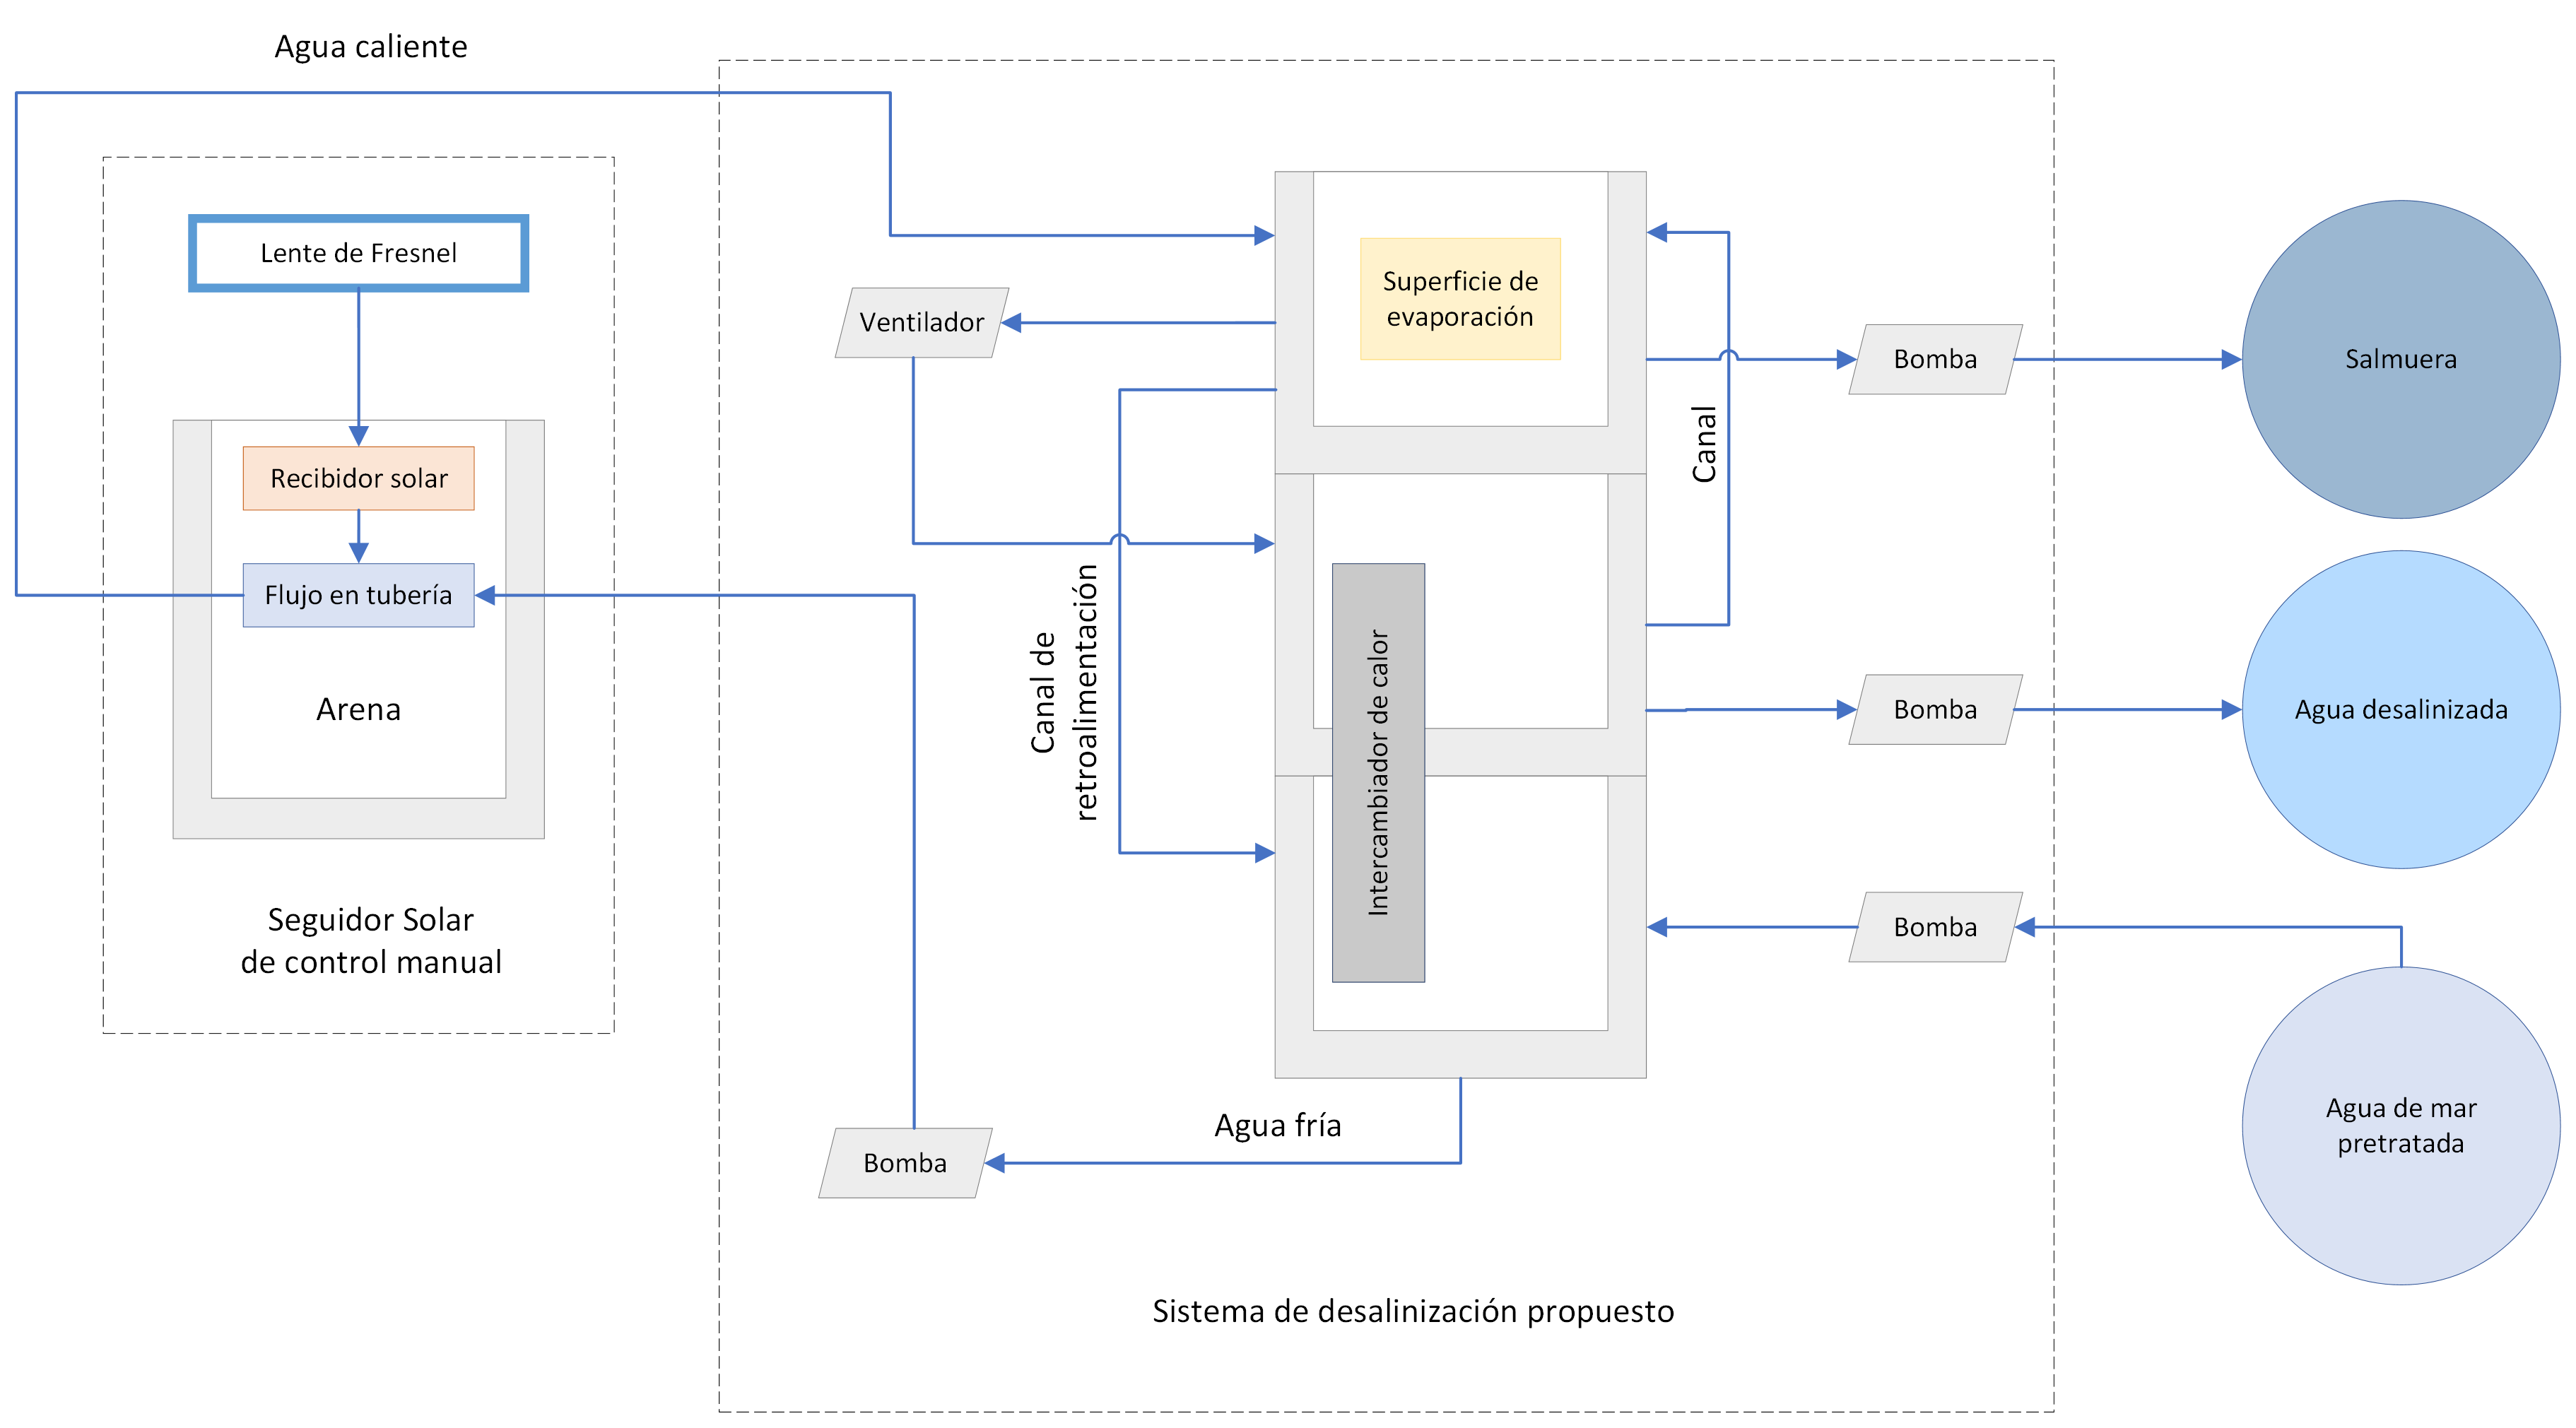
\includegraphics[width=\linewidth, height=12cm, keepaspectratio]{Resultados/Sistema/VistaGeneral.png}
			\caption{Vista general del proceso de desalinización}
			\label{fig:VistaGeneral}
		\end{figure}
		
		Gracias a este esquema se logra evitar la interferencia del vapor de agua a la superficie de calentamiento. Para validar este modelo, se usó Autodesk Inventor para la parte del diseño mecánico del sistema y Autodesk CFD para el modelado de la transferencia de calor y el flujo de aire.
	
		
	
		\subsection{Componentes y módulos del desalinizador}
			
			Tras varias propuestas se llegó a un diseño modular vertical. En la~\cref{fig:WaterModule} se puede observar el primer módulo llamado ``Módulo de reaprovechamiento térmico y bombeo'' el cual se diseñó para aprovechar el calor del vapor generado tras pasar por el ``Módulo de concentración solar'' (\cref{fig:SolarModule}) el cual se integra a un seguidor solar para calentar el agua indirectamente por medio de la lente de Fresnel.
		
		
			\begin{figure}[H]
				\centering
				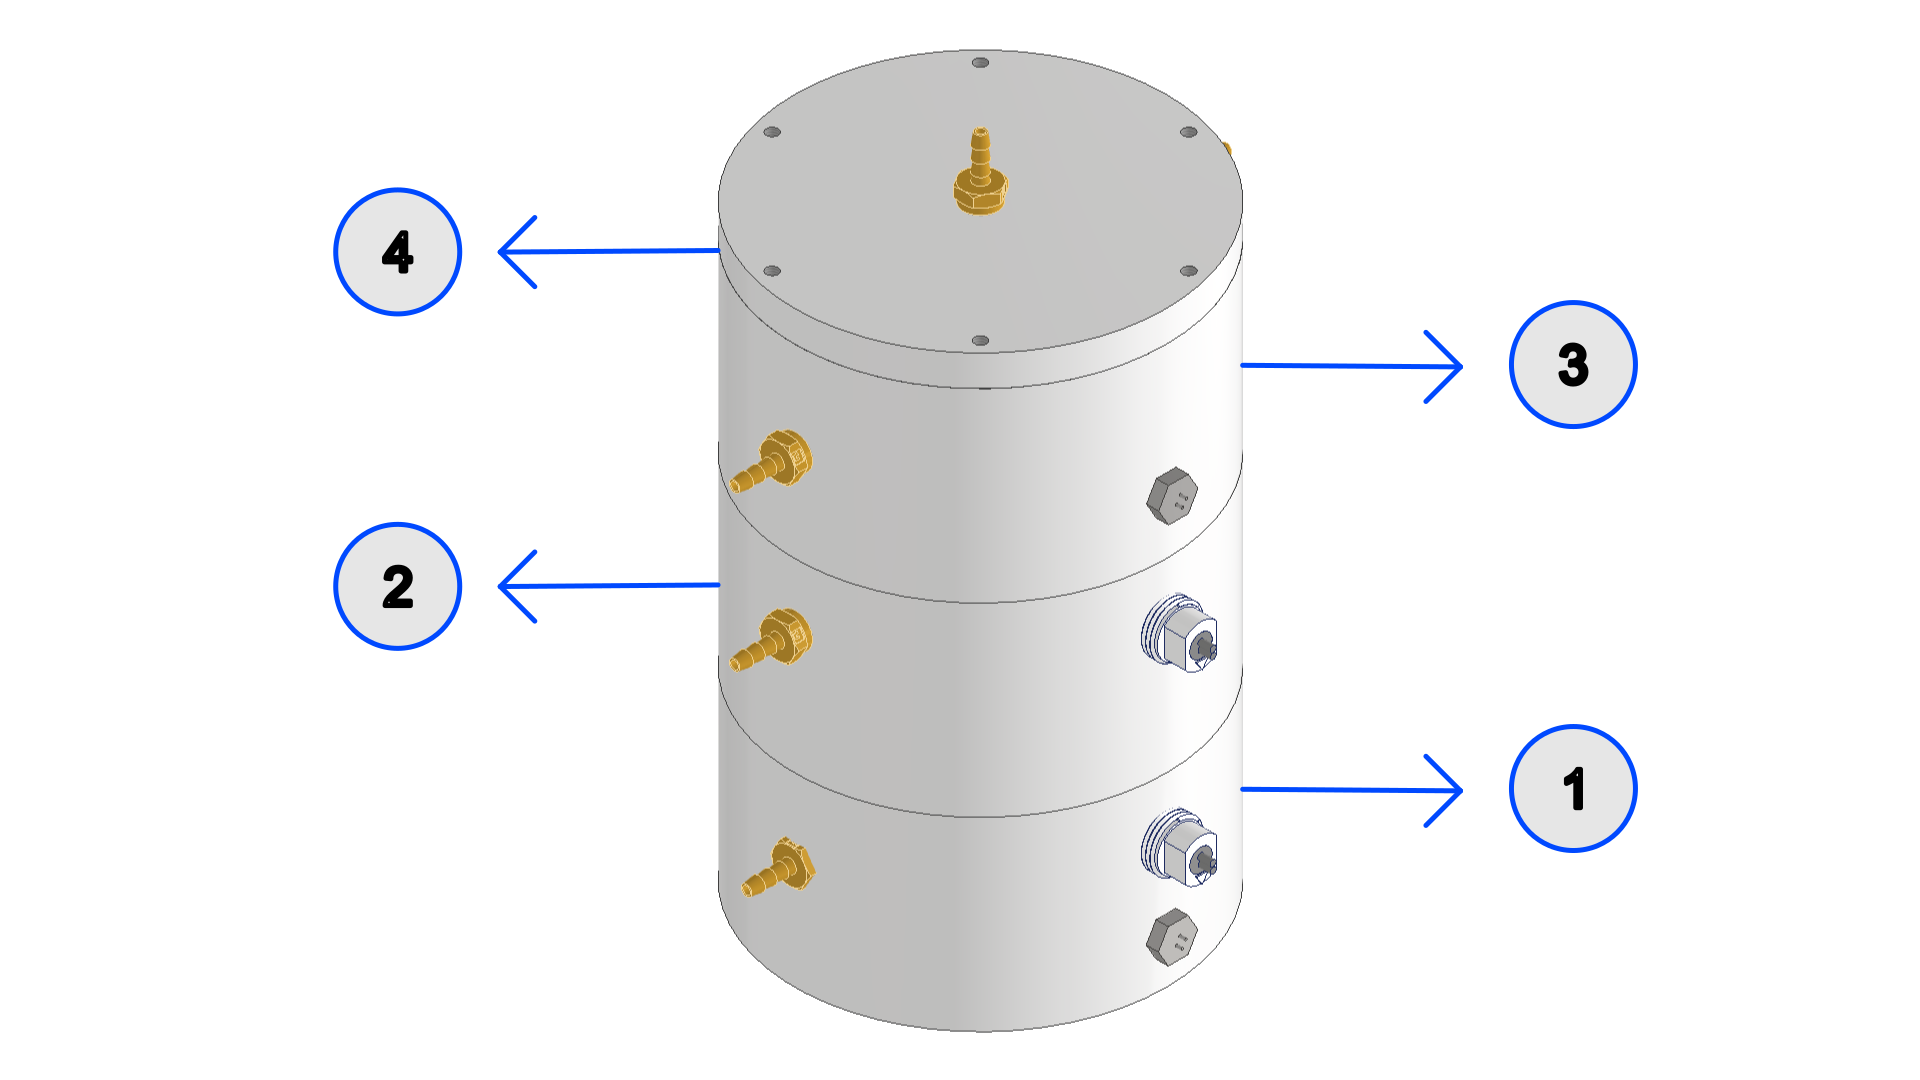
\includegraphics[
					width=\linewidth,
					height=70mm,
					keepaspectratio
				]{Resultados/Sistema/WaterModule.png}
				\caption{Propuesta del sistema desalinizador. Módulo de reaprovechamiento térmico y bombeo.}
				\label{fig:WaterModule}
			\end{figure}
			
			\begin{enumerate}[columns=2]
				\item Contenedor de agua de mar
				\item Contenedor de agua destilada
				\item Cámara de evaporación
				\item Tapa
			\end{enumerate}
			
			\begin{figure}[H]
				\centering
				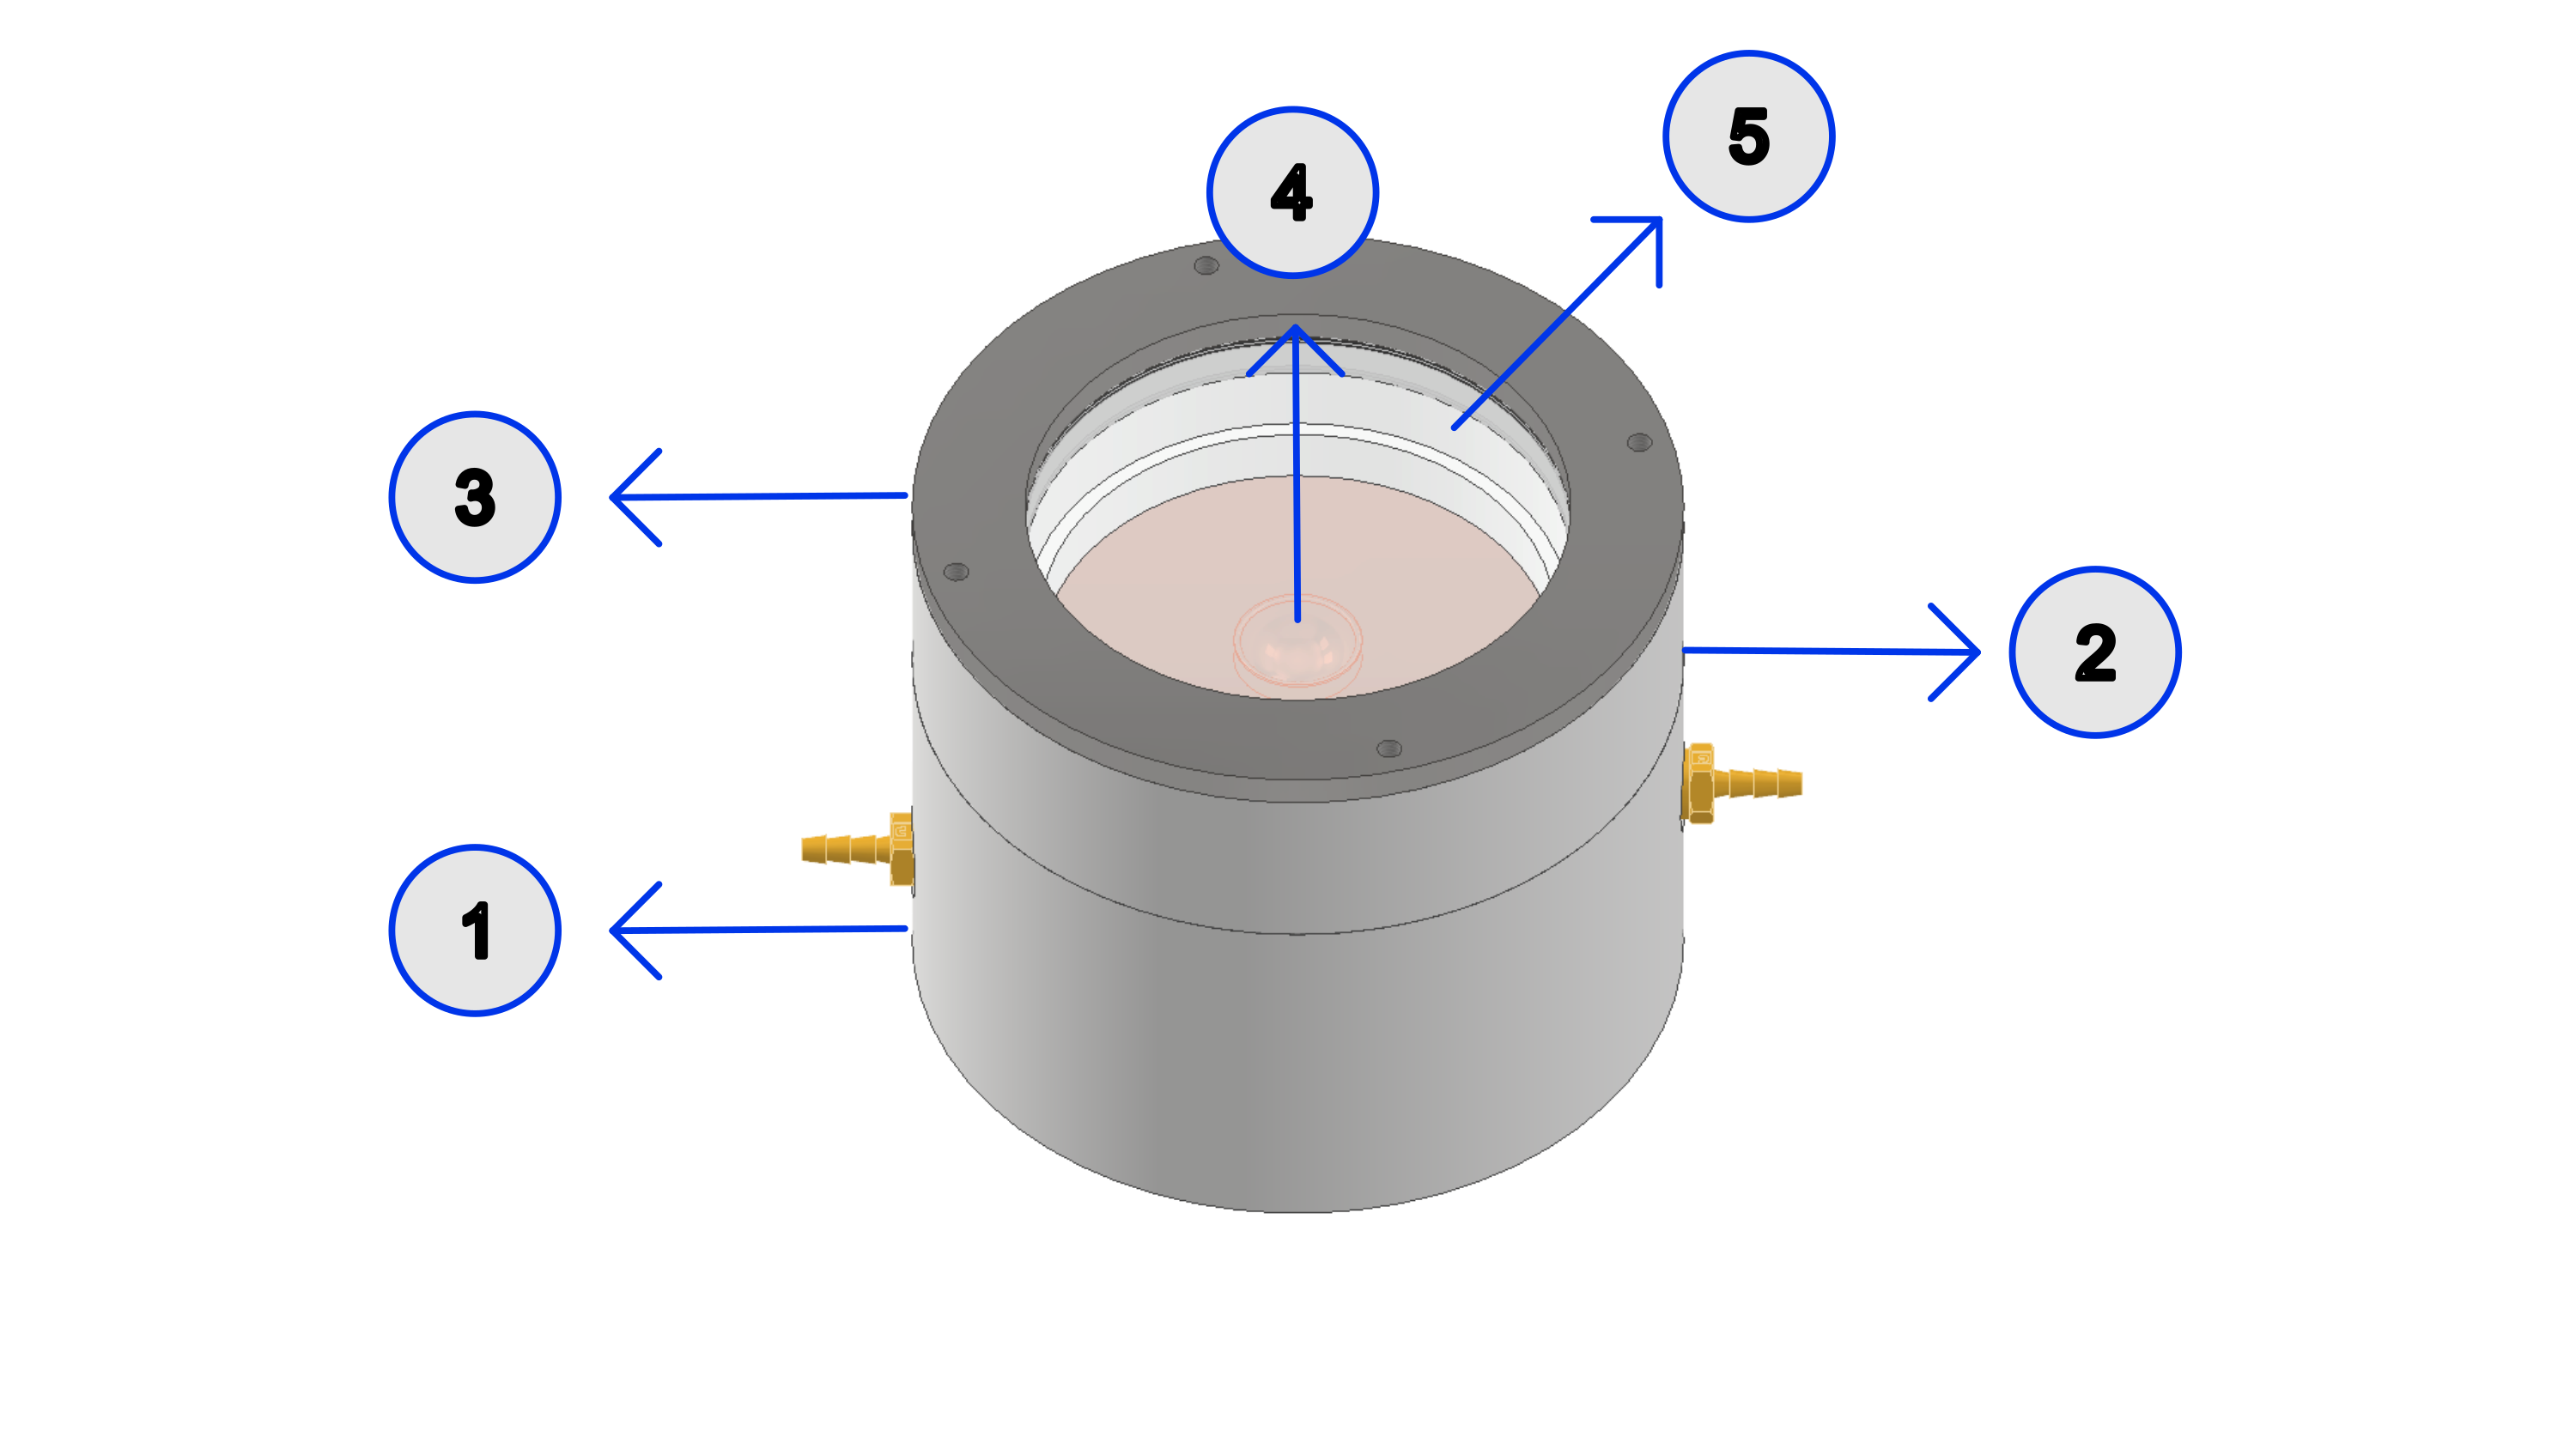
\includegraphics[
					width=\linewidth,
					height=70mm,
					keepaspectratio
				]{Resultados/Sistema/SolarModule.png}
				\caption{Propuesta del sistema desalinizador. Módulo de concentración solar.}
				\label{fig:SolarModule}
			\end{figure}
			
			\begin{enumerate}[columns=2]
				\item Cámara de transferencia de calor
				\item Soporte de lente
				\item Tapa
				\item Recibidor solar
				\item Cristal de borosilicato
			\end{enumerate}
			
			En los siguientes apartados se detallan los elementos que componen a este sistema y las funciones que desempeñan.
	
			\subsubsection{Contenedor de agua de mar}
				
				Su función básica es contener el agua a desalinizar y servir al mismo tiempo como fuente de frío para la condensación del vapor.
				
				El contenedor de agua de mar consta de 2 entradas y 1 salida.
				\begin{itemize}[columns=2]
					\item Entrada de agua de mar
					\item Entrada del excedente de agua caliente
					\item Salida hacia el calentador solar
				\end{itemize}
				
				\begin{center}
					En este módulo se monitorea la temperatura y el nivel del agua.
				\end{center}			
			
			\subsubsection{Contenedor de agua destilada}
				
				Su función básica es promover la condensación del vapor y favorecer el aumento de la temperatura del agua de entrada usando un intercambiador de calor entre la misma cámara y el contenedor de agua de mar.
				
				Este submódulo consta de 1 entrada y 2 salidas.
				
				\begin{itemize}[columns=2]
					\item Entrada de vapor caliente \columnbreak
					\item Salida para regular la presión entre cámaras
					\item Salida de agua destilada
				\end{itemize}
				
				\begin{center}
					En este módulo se monitorea el nivel del agua.
				\end{center}
							
			\subsubsection{Cámara de evaporación}
				
				Su función básica es favorecer el proceso de evaporación aumentando el área superficial por unidad de volumen. Para incrementar la evaporación efectiva se acopló un ventilador que permite desalojar el aire saturado además de promover el flujo del aire.
				
				En una segunda revisión se formuló la posibilidad de agregar elementos que permitieran aumentar el área de contacto del agua con el aire debido a que en realidad se trata de un espacio reducido, por lo que se propone el diseño visto en la~\cref{fig:EvaporationSurface}
				
				\begin{figure}[H]
					\centering
					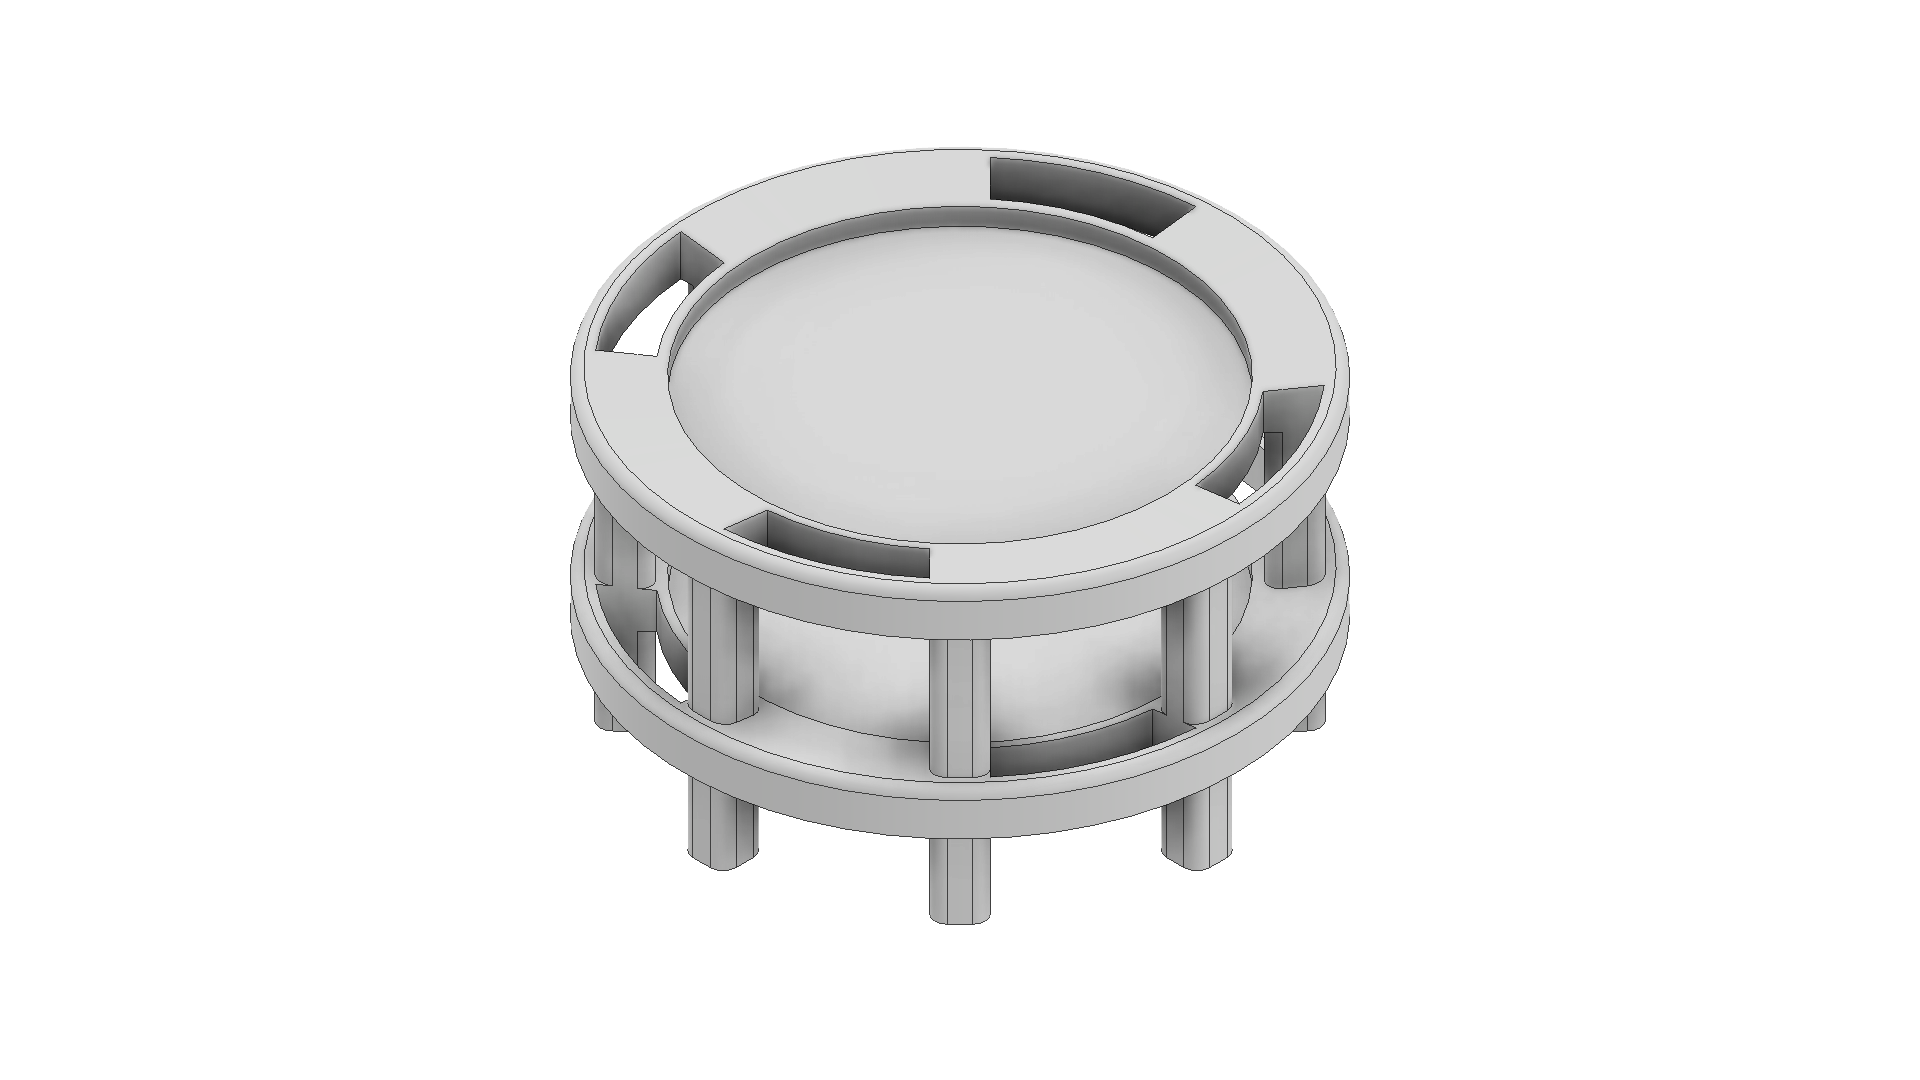
\includegraphics[
						width=\linewidth,
						height=70mm,
						keepaspectratio
					]{Resultados/Sistema/EvaporationSurface.png}
					\caption{Diseño sugerido para aumentar el área de evaporación dentro de la cámara}
					\label{fig:EvaporationSurface}
				\end{figure}
				
				Este submódulo consta de 2 entradas y 2 salidas.
				
				\begin{itemize}[columns=2]
					\item Entrada de agua caliente
					\item Entrada de aire de recirculación
					\item Salida de vapor caliente
					\item Salida de salmuera
				\end{itemize}
				
				\begin{center}
					En este módulo se monitorea la temperatura del agua.
				\end{center}
			
			\subsubsection{Módulo de concentración solar}
				
				Este módulo se divide en dos partes por cuestiones de ensamble y manufactura. La parte superior se encarga de soportar un cristal de borosilicato por el cual atraviesan los rayos solares. Este cristal nos permite mantener un mejor aislamiento térmico del recibidor solar así como evitar la exposición directa al ambiente.
				
				Por otra parte, en el submódulo inferior ocurre el intercambio de calor entre el recibidor solar y el agua. Esto se logra por medio de la conducción de calor entre el recibidor y una tubería de cobre. La elección de la tubería de cobre se dió debido a su alta conductividad térmica, flexiblidad, disponibilidad y costos, ya que en un inicio se planteó el uso de acero galvanizado y de acero inoxidable 316, sin embargo, como se mostrará en las simulaciones siguientes no resultaba buen conductor térmico además de ser difícilmente manufacturable; también se descartó el uso de tuberías de aluminio 5052 debido a su escaza disponibilidad.
				
				
				Este submódulo consta de 1 entrada y 1 salida.
				
				\begin{itemize}[columns=2]
					\item Entrada de agua fría
					\item Salida de agua caliente
				\end{itemize}
				
				\begin{center}
					En este módulo se monitorea la temperatura del recibidor solar.
				\end{center}
		
		\subsection{Simulaciones}
			
			Se realizaron varias simulaciones de transferencia de calor con el fin de validar los diseños propuestos, los materiales seleccionados y el caudal propuesto durante el desarrollo experimental. A su vez, se realizaron simulaciones del flujo de aire en la cámara de evaporación con el fin de validar el diseño visto en la~\cref{fig:EvaporationSurface}.
	
	\section{Control del sistema}
	
		Tras el estudio y comparación de las ventajas y desventajas de diferentes métodos de control numérico se concluyó que el método de control difuso se acoplaba mejor a las necesidades del sistema ya que:
		
		\begin{itemize}
			\item El modelo de contro difuso permite hacer razonamientos para evaluar el grado de certidumbre de una afirmación en vez de limitarse a una lógica binaria donde se producen saltos de una afirmación a otra.
			\item Permite crear un modelo de control basado en reglas fácilmente interpretables
			\item No requiere un modelo matemático u aproximación numérica del proceso, sino, en conocimiento empírico, lo cual es muy beneficioso, ya que tanto el proceso de evaporación como el de ebullición es un fenómeno muy complejo y difícilmente modelable.
			\item Permite tomar decisiones de conocimientos y datos inexactos de forma similar al razonamiento humano
		\end{itemize}
		
		\subsection{Sensores y componentes, calibración y caracterización}\label{subsec:calibración}
		
			En esta sección se detalla el proceso de ajuste y caracterización de los sensores y la bomba que regula el flujo de agua, estas calibraciones resultan indispensables para el correcto funcionamiento del método de control.
			
			\textbf{Termistores}\par
			
			Para caracterizar los termistores se refirió a un set de datos que reflejan la respuesta óhmica al aplicarse cierta temperatura; el código visto en~\cref{ch:steinhart-code}	nos permite hallar los coeficientes de Steinhart-Hart para este modelo.
			
			Se halló que:
			
			\begin{itemize}[columns=3]
				\item A = \num{0.00112866}
				\item B = \num{0.00023422}
				\item C = \num{8.7159e-8}
			\end{itemize}
			
			\textbf{EZO-PMP}\par
			
			La bomba peristáltica EZO-PMP permite una calibración manual, para ello se recreó la configuración vista en la~\cref{fig:Calibración-bomba}
			
			
			\begin{figure}[H]
				\centering
				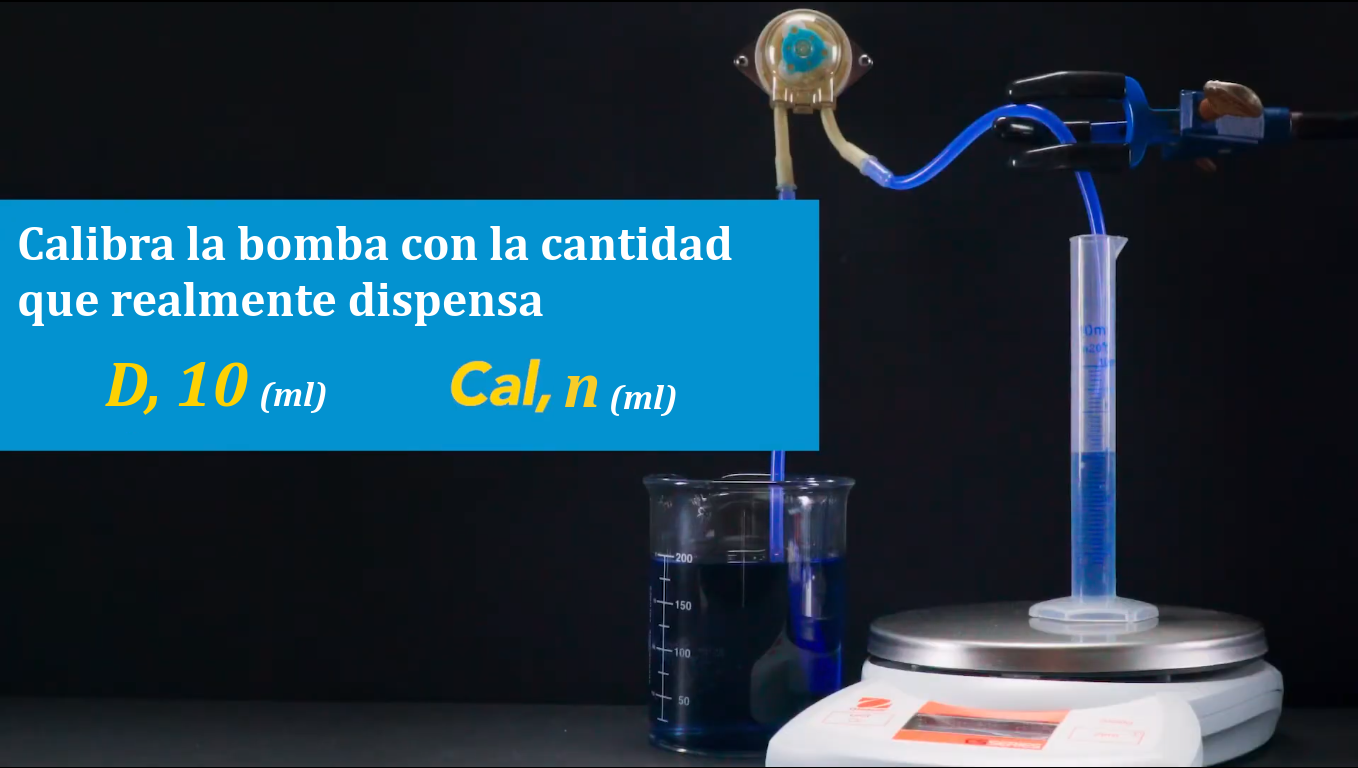
\includegraphics[
					width=\linewidth,
					height=65mm,
					keepaspectratio
				]{Resultados/Control/PumpCalibration.png}
				\caption{Arreglo para la calibración de la bomba EZO-PMP}
				\floatfoot{Imagen adaptada de \cite{atlas_scientific_llc_ezo-pmp_2020}}
				\label{fig:Calibración-bomba}
			\end{figure}
			
			